\chapter{Comparision between "With" and "Without University Degrees?"}

According to Forbes, Most people with data science job titles don’t have these new degrees. I also looked at the profiles of a few data scientist in my Linkedin Network and observed that not all of them have data science degrees. People tend to take different paths - some have degrees in business, economics, maths etc, while some have specialed data science degrees, and some have no university degree. But all of them are working in good organizations with good job roles. In the next section, let's look at the key insights from the Survey Data Analysis. The focus of the analysis is to compare the two groups - individuals who completed university degree vs those without for becoming a data scientist and identify key differences (if any).

Mainly, We will look at two perspectives: Are there a fairly equal percentage of individuals from two groups:
\begin{itemize}
    \item With every compensation bracket.
    \item For each type of job role or activity.
\end{itemize}
\newpage
\section{Compensation}
\begin{figure}[!htpb]
    \centering
    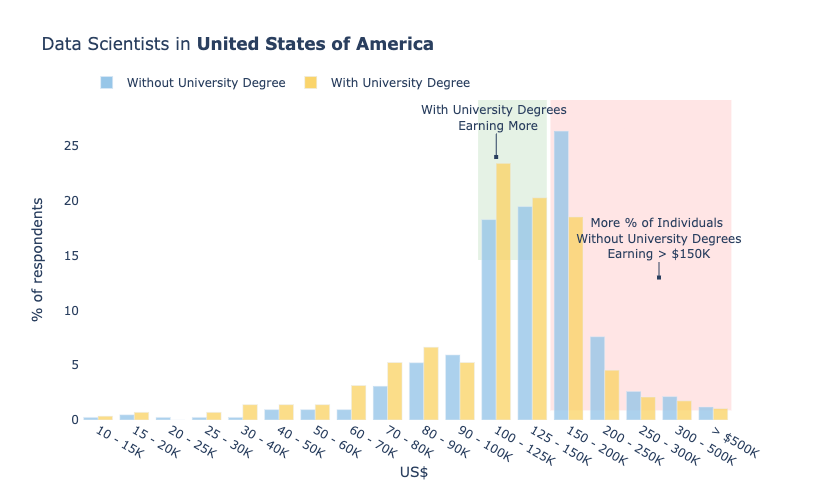
\includegraphics[width=\linewidth]{Figures/Outputs/compensation.png}
    \caption[Compensation]{Compensation}
    \label{fig:figure-06}
\end{figure}
\subsubsection{Key Findings}
The plot shows the percentage of respondents from the United States of America in each compensation bracket. Looking at every bucket, it is clear that there are no significant differences between the two groups. Approximately they differ by a few per cent (less than 5). However, a few sections in this chart are very interesting.
\begin{importantbox}
    A common belief about university degrees is that one get higher compensation. The chart shows that there is a large percentage of individuals \textbf{without a university degree also earning more than 100K USD}. Even without university degrees, if individuals manage to obtain the right skills and the right direction, one can also grab high compensation. That's where Kaggle Learn or Coursera are the best options. As they provide the pathway to get the appropriate skills required to become a data scientist.
\end{importantbox}
There are slight differences when the compensation is less than 125K. For this range, there is a higher percentage of individuals having university degrees. The area is shown in the green section in the chart. Well, this compensation range is the average of most of the companies in USA. This means that university degrees in data science can give an initial boost to the candidates in the compensation.
\begin{importantbox}
    Very Interesting to note that there are more percentage of respondents without university degrees than those who have who are earning in the range of USD 150K-300K. This area is highlighted in red. This implies that there are definately ways to get higher compensation not necessarily after obtaining a masters in data science degree. The obvious reasons can be the amount of experience, age group, or special talent. It will be interesting to specifically look into this cohort where data scientists earn >150K USD. This is analysed in the next section.
\end{importantbox}

\subsection{Key Characteristics : Data Scientists earning > 150K}
The following graph shows the key characteristics: age distribution, coding experience (in years) etc. for Data Scientist earning more than 150K USD.
\begin{figure}[!htpb]
    \centering
    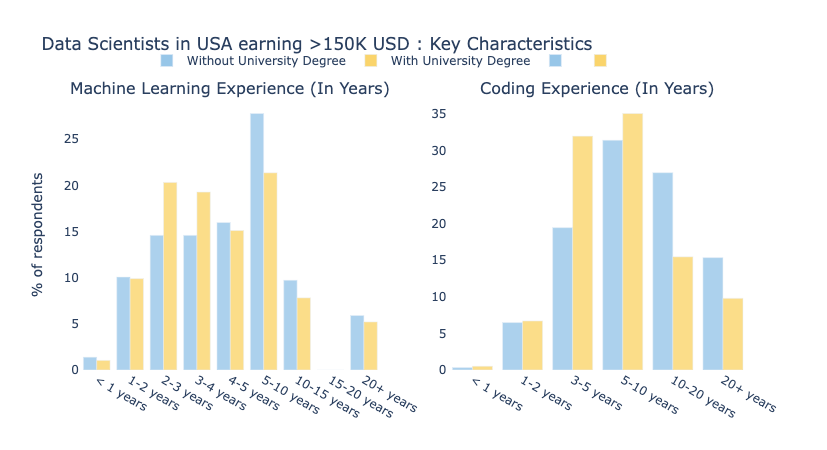
\includegraphics[width=0.8\linewidth]{Figures/Outputs/experience-150.png}
    \caption[Experience of data scientists]{Experience of data scientists earning more than 150K USD.}
    \label{fig:figure-07}
\end{figure}
\begin{figure}[!htpb]
    \centering
    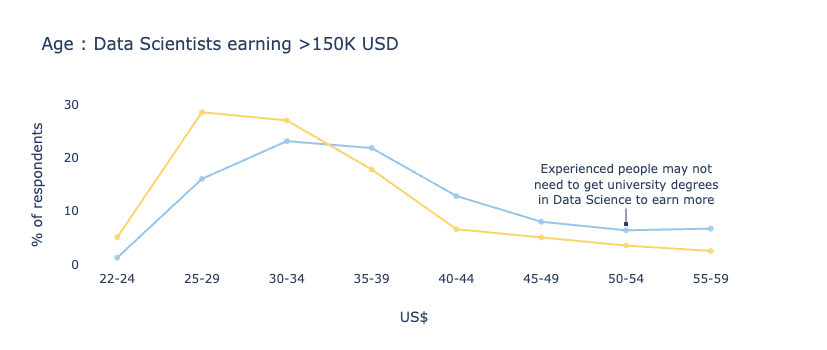
\includegraphics[width=0.77\linewidth]{Figures/Outputs/age-150.png}
    \caption[Age of data scientist]{Age data scientists earning more than 150K USD.}
    \label{fig:figure-08}
\end{figure}

\subsubsection{Key Findings}
\begin{enumerate}
    \item The chart shows that there is a considerable number of individuals in each bracket of the machine learning experience, coding experience, and age. The charts are also does not shows any skewness in a particular bracket.
    \item With more number of years in experience for coding and machine learning (greater than 5), We see that relatively a higher percentage of people are there earning more than 150K without university degrees.
    \item More number of individuals who are aged less than 34 years and with a university degree earn greater than 150K. Good to see that even more percentage of young individuals, aged 22-24 also get higher compensation in the USA.
    \item The portion on the right side of the age graph shows that experienced people may not need to get university degrees in data science if they are only looking for better salaries.
    \item These trends are also similar in other countries. According to many \href{https://www.mastersportal.com/articles/2608/top-9-countries-with-the-highest-investments-in-university-education.html}{links}, top countries for higher education university degrees are the USA, Germany, Canadas etc.
\end{enumerate}
\begin{figure}[!htpb]
    \centering
    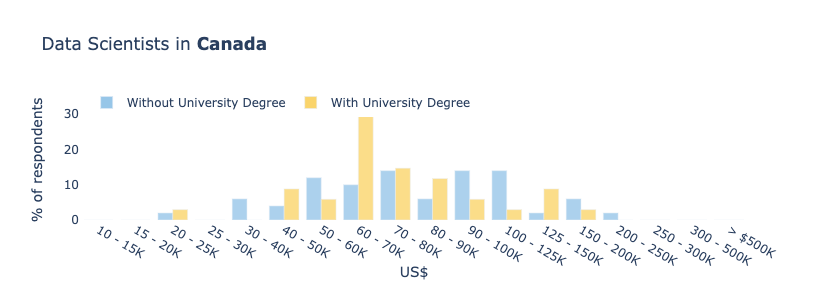
\includegraphics[width=0.8\linewidth]{Figures/Outputs/canada.png}
    \caption[Experience of data scientists in Canada]{Experience of data scientists earning more than 150K USD in Canada.}
    \label{fig:figure-09}
\end{figure}
\begin{figure}[!htpb]
    \centering
    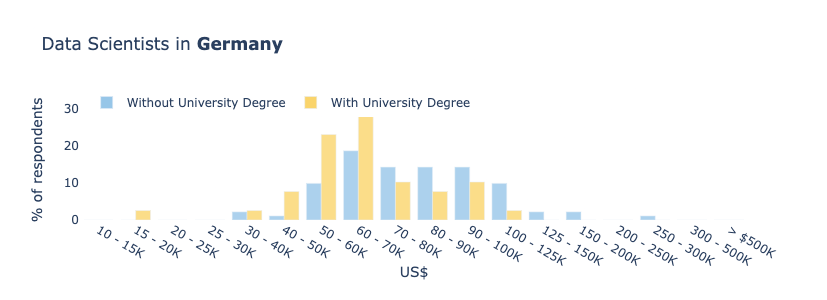
\includegraphics[width=0.8\linewidth]{Figures/Outputs/germany.png}
    \caption[Experience of data scientists in Germany]{Experience of data scientists earning more than 150K USD in Germany.}
    \label{fig:figure-10}
\end{figure}
We see similar insights for these countries as the USA where more percentage of non degree holder respondents are earning higher compensation in many brackets.

\section{Job Role}
Next we look at the job roles of individuals. Does it make a difference in terms of what kind of activity the data scientists do on the daily basis if they are coming with a university degree as compared to without.
\begin{figure}[!htpb]
    \centering
    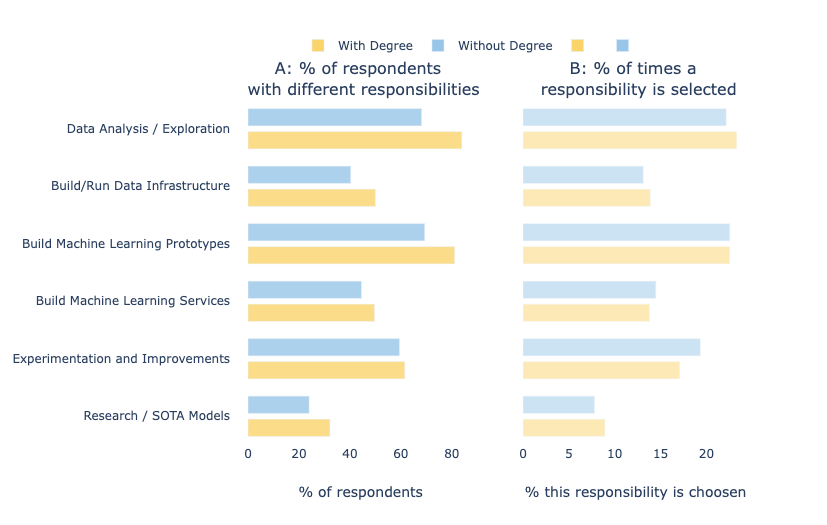
\includegraphics[width=\linewidth]{Figures/Outputs/roles.png}
    \caption[Roles of data engineers]{Roles of data engineers.}
    \label{fig:figure-11}
\end{figure}

The two plots capture two different pieces of information:
\begin{importantbox}
    \textbf{Plot A} shows what percentage of respondents selected a particular activity which people do in their day to day activities. This plot shows which are the most common activities people do in their data science project and the difference between a degree and non-degree holders.
\end{importantbox}
\begin{importantbox}
    \textbf{Plot B} shows, out of all the selected choices by all the respondents, what percentage is a particular responsibility is selected. This plot shows, for a particular group (degree or non-degree holders), which activity has more importance. For example, If a particular 'responsibility' is rarely selected, then the overall percentage will be smaller and If it is selected most of the times, then its overall percentage will also be higher. Meaning that it will be important to the particular group - degree or non-degree holders.
\end{importantbox}
\subsubsection{Key Findings}
\begin{enumerate}
    \item Plot A shows that a higher percentage of individuals with a university degree are involved in different tasks. The biggest differences are observed for data scientists who do "Data Analysis or Exploration", and performing "Research and developing State of the art models". Since experimentation is always a big part of any data science project, there exists very less differences in the \% of respondents of two groups.
    \item The percentage of non-degree holder respondents is always lesser than the counterpart, however, the differences are not extreme. There is still a significant percentage of people who are involved in similar responsibilities as the university holders. Hence, it will be wrong to say that only university holders do a particular type of activities or have specialized activities.
    \item Plot B shows a higher percentage of people with university degrees selected being involved in \textbf{Research work, Data Analysis, and Building/Running Infra-structures}. While a slightly more percentage of people without university degrees selected being involved in Experimentation and Building Machine Learning services.
    \item A fairly equal percentage is observed for people who build Machine Learning service despite their degrees. This particular selection shows that there is no major difference in the kind of work a data scientist will do.
\end{enumerate}

\begin{figure}[!htpb]
    \centering
    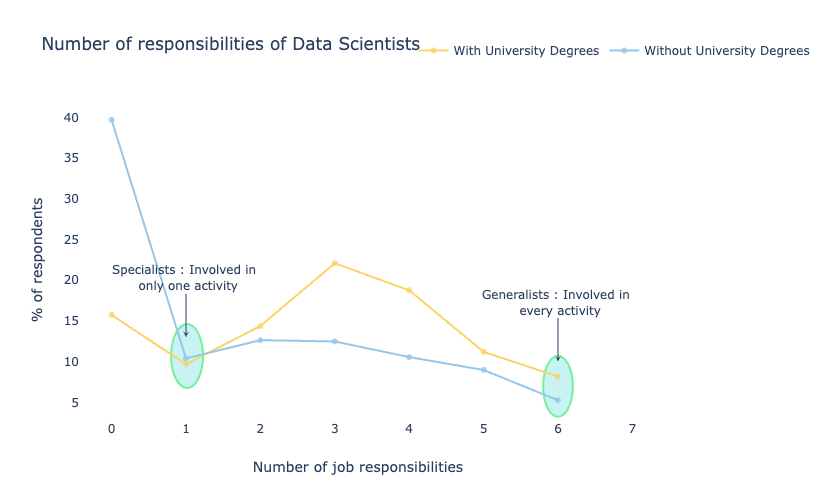
\includegraphics[width=\linewidth]{Figures/Outputs/responsibilities.png}
    \caption[responsibilities of a data scientist]{responsibilities of a data scientist.}
    \label{fig:figure-12}
\end{figure}
\subsubsection{Key Findings}
\begin{enumerate}
    \item Based on the number of job responsibilities, a data scientist can be classified into two categories - Generalist and Specialist. Generalist are the individuals involved in all parts of life cycle of a data science project (ie. the points on the extereme right). Specialists are the individuals who are focussed on hardly 1 or 2 job responsibilities, ie. (points in the left).
    \item We see that slightly more percentage of generalists are there having university degrees. They are they people who are involved in every step - doing analysis, experimentation, building services, and also research. In general, the plot shows that more percentage of people who completed university degrees are involved in multiple responsibilities.
\end{enumerate}
